

\section{Neural Networks}
Artificial Neural Networks are computational models inspired by the structure and functionality of biological brain. They are designed to learn complex relationships from data and have become a fundamental component of modern machine learning. Neural Networks are capable of approximating highly nonlinear functions and are therefore widely used in applications such as image recognition, natural language processing, forecasting, and control systems. There exist various types of neural network architectures, including \acfp{CNN}, \acfp{RNN}, or Transformer models, each tailored to specific types of data and tasks. The following sections provide an overview of the basic building blocks of neural networks, their mathematical formulation, and the training process.


\subsection{Neuron}
The basic element of an artificial neural network is the artificial neuron. The concept is motivated by biological neurons in the human brain, which communicate through electrochemical signals. In a simplified model, a biological neuron receives signals from other neurons through dendrites, processes the received information, and transmits an output signal through its axon \cite{Lin2017ArtificialNN}. Artificial neurons mimic this behavior mathematically by combining several input values into a single output.

\paragraph{History}
The first mathematical model of an artificial neuron was proposed by McCulloch and Pitts in 1943 \cite{McCulloch1990ALC}. Their model consisted of a binary threshold unit that produced an output only when the weighted sum of its inputs exceeded a predefined threshold. Although this model did not include a learning mechanism, it established the foundation for later neural network research.

A major extension of this idea was introduced by Rosenblatt in 1958 with the perceptron \cite{Rosenblatt1958ThePA}. In contrast to the McCulloch--Pitts neuron, the perceptron introduced trainable weights and a learning rule, making it possible to adapt the model parameters directly from data. However, the perceptron still relied on a simple threshold-based activation, which produces a linear decision boundary and was therefore limited to linearly separable classification problems \cite{Minsky1969AnIT}.

This limitation was highlighted by Minsky and Papert, who showed that a single perceptron cannot represent functions such as XOR \cite{Minsky1969AnIT}. The development of multilayer neural networks together with differentiable activation functions later overcame this restriction. These advances made it possible to train networks with multiple layers and enabled the modern neural network architectures that are used in deep learning today.

\paragraph{Mathematical Formulation}
\begin{figure}[!h]
	\centering
	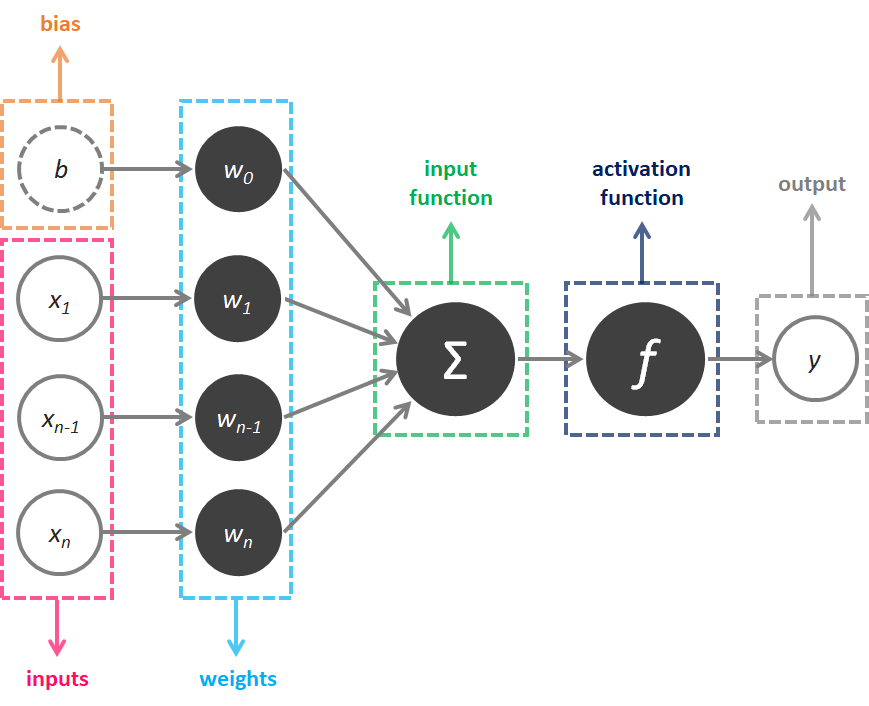
\includegraphics[width=0.6\linewidth]{./chapter2/media/NNNeuron2}
	\caption[Perceptron of an Artificial Neural Network]{Perceptron of an Artificial Neural Network. Image source: \cite{yseYourGuidePerceptrons2024}.}
	\label{fig:NNIntroModernNeuron}
\end{figure}
A neuron receives an input vector $\mathbf{x}=[x_1,x_2,\ldots,x_n]^T$, where each vector element $x_i$ is associated with a trainable weight $w_i$ from the corresponding weight vector $\mathbf{w} = [w_1, w_2, \ldots, w_n]^T$. The neuron first computes a weighted sum of its inputs and adds a bias term $b$, see \autoref{fig:NNIntroModernNeuron}. The resulting pre-activation value is given by: 
% The weighted inputs are summed together with an optional bias term $(b)$, see \autoref{eq:perceptron}. 
\begin{equation}
    z = \sum_{i=1}^{n} w_i x_i + b
    \label{eq:neuron_scalar}
\end{equation}

The value $z$ represents a linear combination of the input features. To enable the modeling of non-linear relationships, an activation function $\phi(\cdot)$ is subsequently applied, yielding the neuron's output:

\begin{equation}
    y = \phi(z) = \phi\left(\sum_{i=1}^{n} w_i x_i + b\right)
    \label{eq:neuron_activation}
\end{equation}

Without the activation function, a composition of multiple neurons would still correspond to a single linear transformation and therefore could not represent complex non-linear patterns. Common activation functions used in modern neural networks include for example the GeLU, tanh (hyperbolic tangent), and ReLU.




The weighted sum in \autoref{eq:neuron_scalar} can be expressed more compactly using vector notation and ending in the form of:
\begin{equation}
    y = \phi\!\left(\mathbf{w}^T \mathbf{x} + b\right)
	= \phi\!\left(
        \begin{bmatrix}
            w_1 & w_2 & \cdots & w_n
        \end{bmatrix}
        \begin{bmatrix}
            x_1 \\
            x_2 \\
            \vdots \\
            x_n
        \end{bmatrix}
        + b
    \right) 
    \label{eq:single_neuron}
\end{equation}

This vector formulation serves as the basis for the matrix representation of an entire neural network layer, where multiple neurons are evaluated simultaneously.

\subsection{Neural Networks}
A neural network is a collection of interconnected neurons organized into layers. 
The input layer receives the feature vector, while the output layer produces the final prediction. The hidden layers between the input and output layers perform intermediate computations that allow the network to learn increasingly abstract representations of the input data \cite{Goodfellow-et-al-2016}.
The parameters of the network, including the weights and biases, are learned from data using optimization algorithms such as gradient descent \cite{Rumelhart1986LearningRB}. The ability of neural networks to learn complex functions from data has made them a powerful tool for a wide range of applications in machine learning and artificial intelligence.

To understand the terminology: Artificial neural network is the broadest term, encompassing all brain-inspired, connectionist models. A feedforward neural network is a subcategory where information flows strictly in one direction (from input to output) without forming cycles, but its layers need not be fully connected \cite{Goodfellow-et-al-2016}. The multilayer perceptron is a feedforward network with one or more fully connected (also called dense) hidden layers, where every neuron in one layer connects to every neuron in the next \cite{Goodfellow-et-al-2016}.
% Each layer consists of multiple neurons, and the output of one layer serves as the input to the next layer.

% In general, a neural network consists of multiple interconnected neurons organized into layers
% , and the output of one layer serves as the input to the next layer. 

\paragraph{Multilayer Perceptron Network}
The most common form of such architectures is the \textit{\acf{MLP}}, also referred to as a feedforward neural network \cite{Goodfellow-et-al-2016}. In an \ac{MLP}, where information flows in one direction from the input layer through one or more fully connected hidden layers to the output layer.  
In an \ac{MLP}, each neuron in a layer receives the outputs of the neurons in the preceding layer as inputs. In a fully connected layer, every neuron is connected to every neuron in the subsequent layer \cite{Goodfellow-et-al-2016}. The output of a layer therefore serves as the input to the next layer.

\begin{figure}[!h]
	\centering
	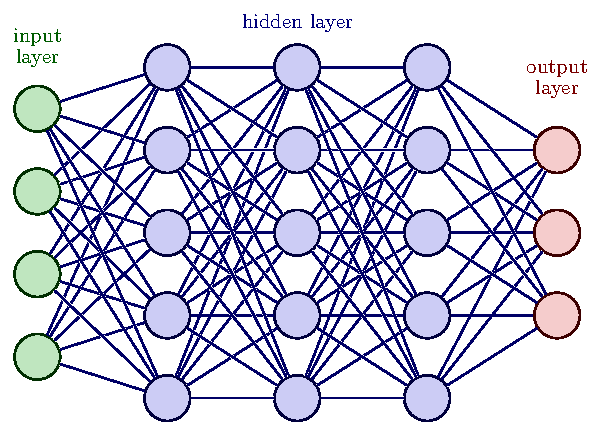
\includegraphics[width=0.6\linewidth]{./chapter2/media/NNNetwork}
	\caption[Neural Networks: Architecture]{Architecture of an Multilayer Perceptron Network. Circles represent perceptrons. Image source: \cite{NeuralNetworksTikZnet2024}.}
	\label{fig:NNNetwork}
\end{figure}


The computation of an entire layer can be expressed compactly using matrix notation. Let $\mathbf{x}^{(l-1)}$ denote the output vector of the previous layer, $\mathbf{W}^{(l)}$ the weight matrix, and $\mathbf{b}^{(l)}$ the bias vector of layer $l$. $M$ are the number of neurons in layer $l$ and $N$ the number of neurons in the previous layer $l-1$. The pre-activation vector is given by:
\begin{equation}
	\mathbf{z}^{(l)} = \mathbf{W}^{(l)} \mathbf{x}^{(l-1)} + \mathbf{b}^{(l)},
\end{equation}
which can be written explicitly as:
\begin{equation}
	\begin{bmatrix}
		w_{11} & \cdots & w_{1N} \\
		w_{21} & \cdots & w_{2N} \\
		\vdots & \ddots & \vdots \\
		w_{M1} & \cdots & w_{MN}
	\end{bmatrix}^{(l)}
	\begin{bmatrix}
		x_1 \\
		x_2 \\
		\vdots \\
		x_N
	\end{bmatrix}^{(l-1)}
	+
	\begin{bmatrix}
		b_1 \\
		b_2 \\
		\vdots \\
		b_M
	\end{bmatrix}^{(l)}
	=
	\begin{bmatrix}
		w_{11}x_1 + \cdots + w_{1N}x_N + b_1 \\
		w_{21}x_1 + \cdots + w_{2N}x_N + b_2 \\
		\vdots \\
		w_{M1}x_1 + \cdots + w_{MN}x_N + b_M
	\end{bmatrix}
\end{equation}

In other words, each neuron in layer $l$ computes its own weighted sum over all outputs of the previous layer and then adds its corresponding bias term. 

Equivalently, the bias can be absorbed into the matrix multiplication by augmenting the input vector with a constant entry $1$ and extending the weight matrix by one additional column:

\begin{equation}
	\begin{bmatrix}
		z_1^{(l)} \\
		z_2^{(l)} \\
		\vdots \\
		z_M^{(l)}
	\end{bmatrix}
	=
	\begin{bmatrix}
		w_{11}^{(l)} & \cdots & w_{1N}^{(l)} & b_1^{(l)} \\
		w_{21}^{(l)} & \cdots & w_{2N}^{(l)} & b_2^{(l)} \\
		\vdots & \ddots & \vdots & \vdots \\
		w_{M1}^{(l)} & \cdots & w_{MN}^{(l)} & b_M^{(l)}
		\end{bmatrix}
		\begin{bmatrix}
		x_1^{(l-1)} \\
		x_2^{(l-1)} \\
		\vdots \\
		x_N^{(l-1)} \\
		1
	\end{bmatrix}
\end{equation}


Then the activation function is applied element-wise to the resulting pre-activation vector $\mathbf{z}^{(l)}$ to produce the output of layer $l$:
\begin{equation}
	\mathbf{x}^{(l)} = \phi(\mathbf{z}^{(l)}) = \phi\!\left(\mathbf{W}^{(l)} \mathbf{x}^{(l-1)} + \mathbf{b}^{(l)}\right).
\end{equation}



\paragraph{Non-Linear Activation Functions in Neural Networks}
The introduction of non-linear activation functions is essential, as a composition of purely linear transformations would again result in a linear model \cite{Goodfellow-et-al-2016}. By combining multiple layers with non-linear activations, neural networks can approximate highly complex functions and learn non-linear, intricate patterns from data \cite{Hornik1991ApproximationCO}. In fact, sufficiently large neural networks are universal function approximators, meaning they can approximate a wide range of continuous functions to arbitrary accuracy. 
Common activation functions used in modern neural networks include the functions GELU (Gaussian Error Linear Unit) \cite{Hendrycks2016GaussianEL}, ReLU (Rectified Linear Unit) \cite{Nair2010RectifiedLU}, Leaky ReLU \cite{Maas2013RectifierNI}, the tanh (hyperbolic tangent) \cite{Ryck2021OnTA} and the Swish function \cite{Ramachandran2017SwishAS}. But there exist many more. Each of these functions has its own characteristics and can result in different learning dynamics and performance. 

% ToDo: Figure to activation functions




\paragraph{Prediction}
The output layer is responsible for producing the network's final prediction. Its activation function is chosen based on the task: 
\begin{itemize}
	\item \textbf{Regression:} For regression problems, a linear activation directly outputs a continuous value.
	\item \textbf{Binary Classification:} For binary classification (true/false), a single neuron with a sigmoid function outputs a probability between 0 and 1.
	\item \textbf{Multi-Class Classification:} For multi-class classification, a softmax layer produces a probability distribution over the classes, where each output neuron corresponds to a specific class and the softmax function ensures that the outputs sum to 1, representing the predicted probabilities for each class.
\end{itemize}
The choice of activation function in the output layer is crucial, as it directly affects the interpretation of the network's predictions and the appropriate loss function to use during training.




\paragraph{Loss Function}
The loss function $\mathcal{L}$ is a measure of how well the network is able to predict the target value and quantifies the difference between the network's predictions and the true labels in the training data. The goal of the training process is to minimize the loss function by adjusting the weights of the network. The loss function can be any differentiable function, but common choices are \acf{MSE} for regression tasks and cross-entropy for classification tasks.
\begin{itemize}
	\item \textbf{\acf{MSE} Loss Function:} Commonly used for regression tasks, where the goal is to predict continuous values. The \acf{MSE} loss function is defined as:
	\begin{equation}
		\mathcal{L} = \frac{1}{N} \sum_{i=1}^{N} (y_i - \hat{y}_i)^2
	\end{equation}
	where $y_i$ is the target value for the $i$-th sample, $\hat{y}_i$ is the predicted value for the $i$-th sample, and $N$ is the number of samples.
	

	\item \textbf{Cross-Entropy Loss Function:} Commonly used for classification tasks, where the goal is to predict discrete class labels. 
	\begin{itemize}
		\item \textit{Binary Classification:} For binary classification problems, the network typically uses a single output neuron with a sigmoid activation. The output $\hat{y}_i \in [0,1]$ represents the predicted probability of the positive class. The binary cross-entropy loss is then defined as:
		\begin{equation}
			\mathcal{L} =
			-\frac{1}{N}\sum_{i=1}^{N}
			\left(
			y_i \log(\hat{y}_i) + (1 - y_i)\log(1 - \hat{y}_i)
			\right)
		\end{equation}
		where $y_i \in \{0,1\}$ denotes the true label of the $i$-th sample, $\hat{y}_i$ is the predicted probability of the positive class, and $N$ is the number of samples.

		\item \textit{Multi-Class Classification:} For multi-class classification problems with $C$ classes, the network output is typically normalized using a softmax function to obtain a probability distribution over all classes (which sums up to 1 over the classes). The corresponding cross-entropy loss is defined as:
		\begin{equation}
			\mathcal{L} =
			-\frac{1}{N}\sum_{n=1}^{N}\sum_{i=1}^{C}
			y_{n,i}\log(\hat{y}_{n,i})
		\end{equation}
		where $y_{n,i}$ represents the one-hot encoded ground-truth label and $\hat{y}_{n,i}$ is the predicted probability for class $i$ of sample $n$.
	\end{itemize}

\end{itemize}
















\subsection{Training Neural Networks}
% gradient based optimization
The parameters of a neural network, namely the weights and biases, are learned from data during training. This is typically achieved by minimizing a loss function $\mathcal{L}$ using optimization methods such as \textit{gradient descent} and its variants. The gradients required for optimization are efficiently computed using the \textit{backpropagation} algorithm, which propagates the prediction error from the output layer back through the network \cite{Rumelhart1986LearningRB}. This learning process enables neural networks to adapt their internal representations and achieve strong performance across a wide range of machine learning tasks.

\paragraph{What is a Gradient?} 
The gradient is a fundamental concept in optimization and machine learning \cite{Rumelhart1986LearningRB, Bottou2016OptimizationMF}. It describes how a function changes with respect to its input variables and points in the direction of the steepest increase of the function. In the special case of a function with only one variable, the gradient reduces to the first derivative, which corresponds to the slope of the function at a given point.
In simple terms, the gradient indicates how the function value changes when making a small step to the right or left away from a specific point.



% In Figure~\ref{fig:NNGradientIntro}, the gradient is represented by the slope of the curve at a particular point. It indicates how the function value changes when moving slightly away from that point.
% The gradient is represented by the slope of the curve at a particular point. 

To better understand the concept of gradients, consider \autoref{fig:NNGradientIntro}. We want to determine the slope of the blue curve at the point $x=1$. To do this, we calculate the gradient at that point. First, we compute the derivative $f'(x)=2x$ of the function $f(x)=x^2-3$ and evaluate it at $x=1$. The first derivative $f'(x)$ provides the slope at any point on the function $f(x)$. In this example, the slope at $x=1$ is $f'(1)=2$. To verify this result, the slope triangle is shown in \autoref{fig:NNGradientIntro}. It provides a visual representation of the slope and confirms the calculated value of with the slope $m=2$.

\begin{figure}[!h]
	\centering
	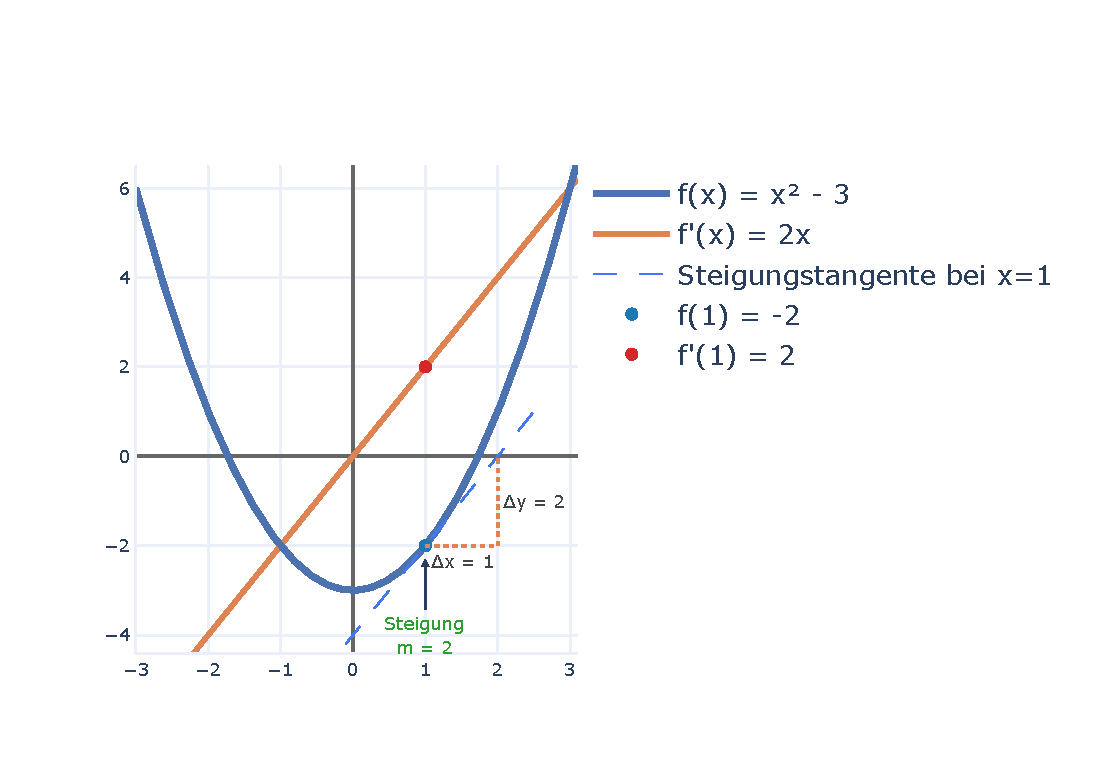
\includegraphics[width=0.85\linewidth]{./chapter2/media/NNGradientIntro.pdf}
	\caption[Understanding Gradients]{Understanding Gradients: The gradient of a 1D function $f(x)$ at point $x=1$ is calculated with the derivative $f'(x)$. It represents the slope of the tangent line at that point.}
	\label{fig:NNGradientIntro}
\end{figure}

In general, the gradient indicates whether a function is increasing or decreasing at a specific point and how steeply it changes. A positive gradient means that the function is increasing, while a negative gradient indicates that the function is decreasing. The magnitude of the gradient describes how steeply the function changes. Larger magnitudes correspond to steeper slopes, while values close to zero indicate relatively flat regions.



\paragraph{Gradient Descent and Parameter Update} 
Gradient descent is an iterative optimization algorithm that is used to minimize a loss function \cite{Bottou2016OptimizationMF}.
The basic principle of gradient descent can be understood by considering a simplified setting with a single parameter -- a network weight -- as illustrated in the Figure~\ref{fig:NNGradientDescent_2}. 
The horizontal axis represents the value of the weight, while the vertical axis represents the corresponding loss, which quantifies the discrepancy between the predicted and true values of the training data.

\begin{figure}[!h]
	\centering
	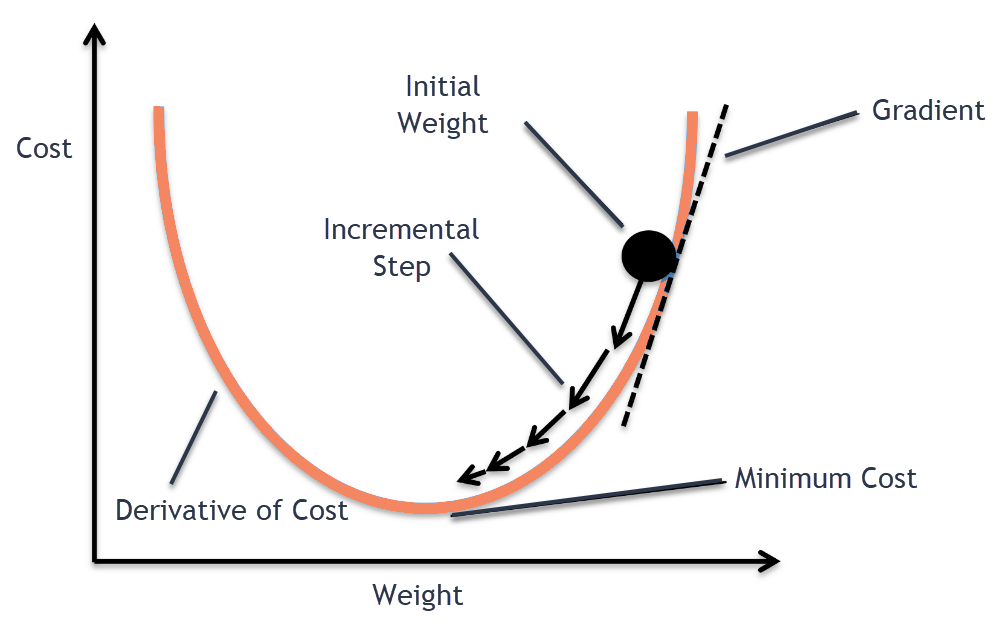
\includegraphics[width=0.6\linewidth]{./chapter2/media/NNGradientDescent_2}
	\caption[Neural Network: Simplified Gradient Descent]{Simplified gradient descent based on one network weight. Image source: \cite{lanhamLearnARCoreFundamentals}.}
	\label{fig:NNGradientDescent_2}
\end{figure}

The resulting curve is the loss landscape for that one parameter. At any point on the loss curve, the derivative (or gradient) indicates the local slope of the function.
% The current network weight, shown by the black dot must be updated in a way, to reduce the loss.
The current value of the weight, represented by the black dot, must be adjusted such that the loss decreases. Gradient descent achieves this through the following two steps:
\begin{enumerate}
	\item \textbf{Calculate the gradient:} 
	Compute the gradient of the loss function with respect to the weight. 
	% The gradient of the loss function with respect to the weight is calculated.
	% The first step is to compute the gradient of the loss function with respect to the weight. 
	The gradient indicates how the loss changes as the weight is adjusted.
	% The gradient of the loss function with respect to the parameter is calculated.
	\item \textbf{Update the weight:} The weight is then updated by moving in the opposite direction of the gradient. 
	Since the gradient points towards the direction of steepest increase, moving against it results in a reduction of the loss.
	% This is because the gradient points in the direction of steepest ascent, so moving in the opposite direction will lead to a decrease in the loss. 
	The basic parameter update is defined as:
	\begin{equation}	
		\mathbf{W}_{\text{t+1}} = \mathbf{W}_{\text{t}} - \alpha \cdot \nabla \mathcal{L}(\mathbf{W}_{\text{t}})
	\end{equation}
	where $\alpha$ denotes the learning rate, which controls the step size of the update, and $\nabla \mathcal{L}(\mathbf{W}_{\text{t}})$ is the gradient of the loss function with respect to the parameter at iteration $t$.
	% where $\alpha$ is the learning rate, a hyperparameter that controls the step size of the update, and $\nabla L(W_{\text{t}})$ is the gradient of the loss function with respect to the weight at its current value.	
\end{enumerate}



In the example shown in Figure~\ref{fig:NNGradientDescent_2}, the gradient is positive. Consequently, increasing the weight would increase the loss.
To reduce the loss, the weight must therefore be moved in the opposite direction (to the left). This procedure is repeated iteratively until the algorithm reaches a minimum of the loss function or another stopping criterion is satisfied. The successive parameter updates are illustrated by the black arrows in Figure~\ref{fig:NNGradientDescent_2}. At the minimum, the gradient and the slope are zero and the parameter update becomes zero as well. The algorithm has converged. 

\textit{Goal of Training Neural Networks:} The goal is to find the optimal set of parameters that minimizes the loss function, which corresponds to the best fit of the model to the data, meaning the network's predictions are sufficiently accurate \cite{Bottou2016OptimizationMF}. 






\paragraph{Optimization Problems}
But not every minimum found is a good solution. The loss landscape of neural networks is highly non-convex and can contain many local minima, saddle points, and flat regions, where the gradient is zero but the loss is not minimized. If the gradient gets zero, the optimization process get stuck \cite{Bottou2016OptimizationMF}. \autoref{fig:NNGradientDescent_2} shows a loss landscape with two parameters. The black dot represents the inital parameter values and the line shows the trajectory of the parameter updates during training. As seen it depends on the initial parameter values, whether the algorithm converges to the global minima, local minama or to the saddle point in the middle of the two hills.  


\begin{figure}[!h]
	\centering
	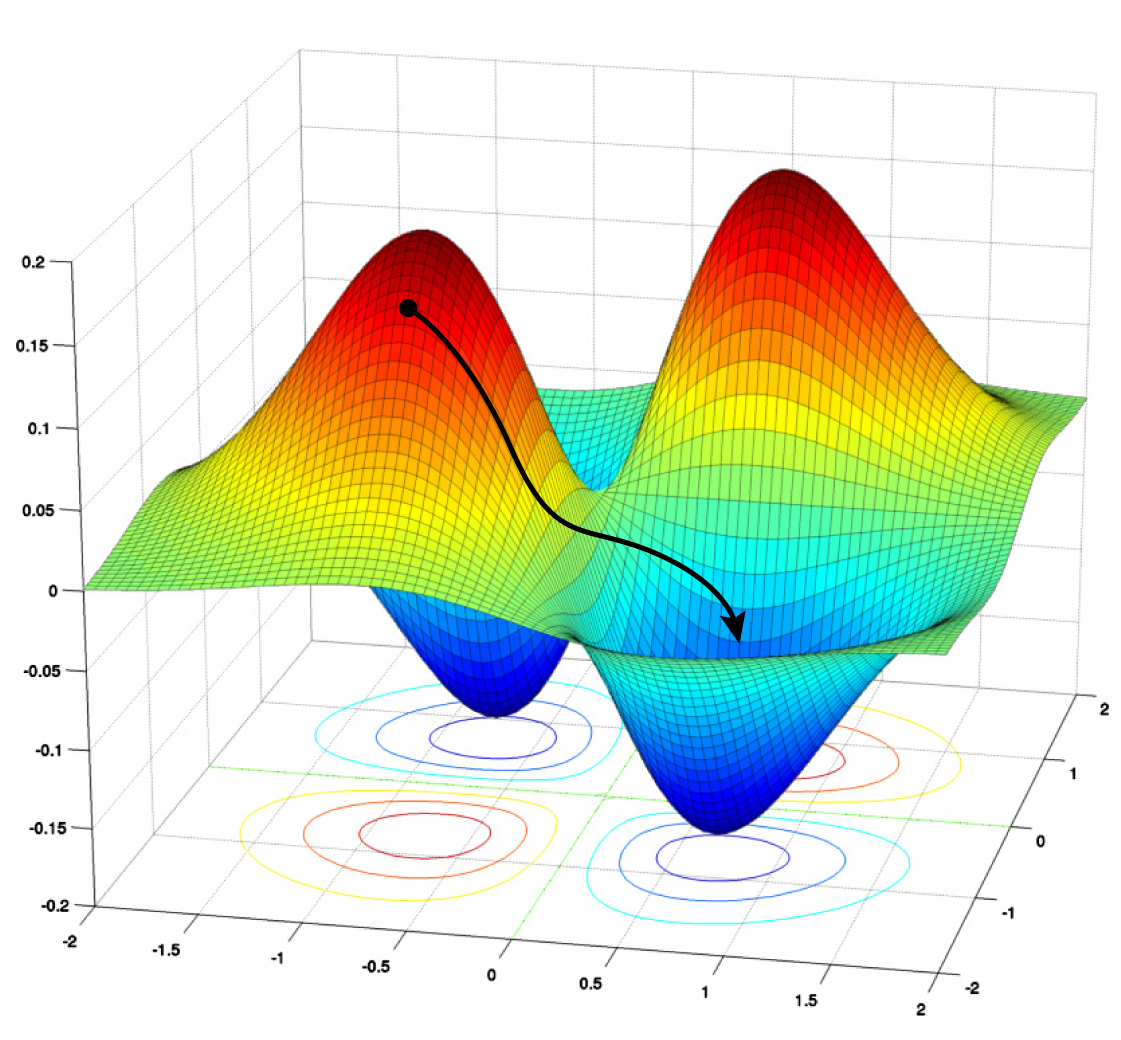
\includegraphics[width=0.52\linewidth]{./chapter2/media/NNGradientDescent}
	\caption[Neural Networks: Optimization Problems]{Neural Networks and their optimization Problems: The figure shows a loss landscape of two parameters, which has a local minima and a saddle point, where the training precess could get stuck. Image source: \cite{ananthaswamyResearchersBuildAI2022}.}
	\label{fig:NNNetwork}
\end{figure}

In the shown examples, the loss landscape was known, but in practice, the loss landscape of neural networks is typically unknown and can be highly complex.  Neural networks often consists of millions of parameters and therefore they have a high-dimensional loss landscape. The Algorithm works in such high-dimensional spaces in the same way.
% The optimization process works in such high-dimensional spaces in the same way and navigates through this loss landscape to find a set of parameters that minimizes the loss function. 
Therefore, training neural networks can be challenging and may require careful tuning of hyperparameters such as the learning rate, as well as the use of techniques like momentum, adaptive learning rates or regularization to improve convergence and generalization performance \cite{Bottou2016OptimizationMF}. For this many variants of the basic gradient descent algorithm have been developed, which is not the scope of this work.


% \textit{Backpropagation.}
% The gradients needed for the parameter updates in gradient descent are computed using the backpropagation algorithm. Backpropagation efficiently propagates the error from the output layer back through the network to compute the necessary gradients for all parameters. For each neuron, the corresponding proportion of the total error is calculated and the weights are adjusted accordingly. 

\paragraph{Backpropagation}
The gradients required for updating the network parameters in gradient descent are computed using the \textit{backpropagation algorithm} \cite{Rumelhart1986LearningRB}. Backpropagation efficiently propagates the prediction error from the output layer back through the network and computes the gradients of the loss function $\mathcal{L}$ with respect to all weights $\mathbf{W}$ in the model. Based on these gradients, each parameter $w_{ij}^l$ is adjusted proportionally to its contribution to the overall error.

More precisely, backpropagation computes the partial derivatives of the loss function with respect to all trainable parameters in the network. These gradients quantify how sensitive the loss is to small changes in each parameter and therefore indicate how each parameter should be adjusted to reduce the overall error. Parameters that contribute more strongly to the error receive larger updates, while less influential parameters are adjusted more mildly.
The training process for a neural network can therefore be summarized by the following update rule:
\begin{equation}
\mathbf{W}_{t+1} = \mathbf{W}_t - \alpha \cdot \nabla_{\mathbf{W}_t} \left( \frac{1}{N} \sum_{i=1}^{N} \mathcal{L}\bigl(\mathbf{y}_i, f_{\mathbf{W}_t}(\mathbf{x}_i)\bigr) \right)
\end{equation}
where $f_{\mathbf{W}}$ denotes the neural network with parameters $\mathbf{W}$, $\mathcal{L}$ is the loss function measuring the difference between the predicted output $f_{\mathbf{W}}(\mathbf{x}_i)$ and the target value $\mathbf{y}_i$, $\alpha$ is the learning rate, $N$ is the number of training samples, and $\nabla_{\mathbf{W}_t}$ represents the gradient of the loss function with respect to the weights at iteration $t$.

By iteratively applying this update rule, the network parameters are gradually adjusted in a direction that reduces the loss function. This iterative optimization process is what allows the neural network to learn meaningful representations from training data and improve its predictions over time.


Besides the standard gradient descent algorithm, which computes the gradient over the entire dataset, several more efficient variants are commonly used in practice. In stochastic gradient descent (SGD), the exact gradient is not evaluated on the full dataset \cite{Bottou2010LargeScaleML, Robbins1951ASA}. Instead, it is approximated using only a single randomly selected training sample at each iteration. A further extension is mini-batch gradient descent, where the gradient is computed on a small subset of the training data (a mini-batch) rather than on a single sample or the full dataset \cite{Bottou2016OptimizationMF, Goodfellow-et-al-2016}. This approach reduces the computational cost per update while still providing a more stable gradient estimate compared to pure stochastic gradient descent.






\subsection{Evaluation}

\paragraph{Evaluation Metrics}
To measure the performance of a machine learning model, various evaluation metrics can be used depending on the specific task and problem setting. These metrics provide quantitative measures of how well a model performs and allow comparisons between different models or configurations. While common examples include accuracy, precision, recall, and the F1-score for classification tasks, as well as mean squared error for regression tasks. However, a detailed discussion of these metrics is beyond the scope of this work.

\paragraph{Evaluation}
The performance of a machine learning model is typically evaluated using data that has not been seen during training, referred to as test data. This allows an unbiased assessment of the model's ability to generalize to new, unseen samples. There exist in general three main scenarios regarding the model's performance on training and test data:
\begin{itemize}
	\item \textbf{Underfitting:} A model that underfits performs poorly on both training and test data. It fails to capture the underlying patterns in the training data, resulting in high error on both datasets.
	\item \textbf{Overfitting:} An overfitted model achieves high performance on the training data but fails to generalize well to the test data. It has essentially memorized the training samples, including noise and outliers, which leads to poor performance on new data.
	\item \textbf{Well-Balanced Model:} A well-balanced model achieves consistently good performance on both training and test datasets. It captures the underlying patterns in the training data without overfitting, allowing it to generalize effectively to unseen samples. 
\end{itemize}

% This is typically done using optimization algorithms such as gradient descent, which is the most common optimization algorithm in practice. The gradients needed for these updates are computed using the backpropagation algorithm, which efficiently propagates the error from the output layer back through the network to compute the necessary gradients for all parameters. For each neuron, the corresponding proportion of the total error is calculated and the weights are adjusted accordingly. Through this process, neural networks can learn complex patterns and achieve high performance on a variety of tasks.



% This process is repeated iteratively, with the weight being updated in each iteration until convergence is achieved, meaning that the loss is minimized and the network's predictions are sufficiently accurate, see the black arrows in Figure~\ref{fig:gradient_descent}.





% , meaning that the loss is minimized and the network's predictions are sufficiently accurate

% First the gradient is calculated. 
% If the derivative is positive (the tangent slopes upward to the right), increasing the weight would increase the cost; conversely, moving the weight in the opposite direction (to the left) reduces the cost. 

% Gradient descent formalizes this intuition by always updating the parameter in the direction opposite to the gradient – that is, downhill along the loss surface.


% The training of a neural network involves adjusting its parameters (weights and biases) to minimize a loss function. The loss function $\mathcal{L}$ is a measure of how well the network is able to predict the target
% value and quantifies the difference between the network's predictions and the true labels in the training data. This is typically done using optimization algorithms such as gradient descent, which is the most common optimization algorithm in practice. 





% To better understand the gradient descent algorithm, consider a 
% Gradient descent iteratively updates the parameters in the direction that reduces the loss.




% Gradient descent is the most common optimization algorithm used in practice. The gradients needed for these updates are computed using the backpropagation algorithm, which efficiently propagates the error from the output layer back through the network to compute the necessary gradients for all parameters. For each neuron, the corresponding proportion of the total error is calculated and the weights are adjusted accordingly. Through this process, neural networks can learn complex patterns and achieve high performance on a variety of tasks.

% . If the predicted output is close to the target, the value of the loss function will be
% small. If the predicted output is far from the target, the value of the loss function will
% be large. The goal of the training process is to minimize the loss function by adjusting
% the weights of the network. The loss function can be any differentiable function, but
% common choices are Mean Squared Error (MSE) for regression tasks and cross-entropy
% for classification tasks. The MSE loss function is defined as:
% Where yi is the target value for the i-th sample, yi
% is the predicted value for the i-th sample, and N is the number of samples. The cross-entropy loss function is defined as:




% A neural network consists of multiple interconnected neurons organized into layers. Typically, the network is composed of an input layer, one or more hidden layers, and an output layer. The input layer receives the feature vector, while the output layer produces the final prediction. The hidden layers perform intermediate computations that allow the network to learn increasingly abstract representations of the input data.